\mode<article>{
	\clearpage
}

\section{Sockets and combined interfaces}

\mode<presentation>{
\begin{frame}
	\frametitle{Sockets and combined interfaces}
	A \emph{socket} is a facility class that combines an export with a port.
	Two different sockets:
	\begin{itemize}
		\item<1-> \textbf{initiator}:
		\begin{itemize}
			\item<1-> port for the forward path
			\item<1-> export for the backward path
		\end{itemize}
		\item<1-> \textbf{target}:
		\begin{itemize}
			\item<1-> export for the forward path
			\item<1-> port for the backward path
		\end{itemize}
	\end{itemize}
	\begin{center}
		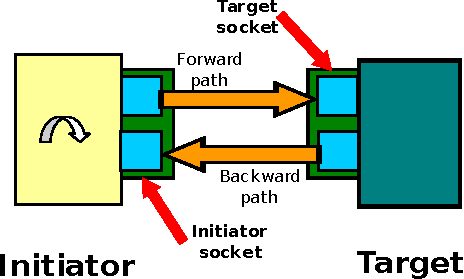
\includegraphics[width=0.6\textwidth]{tlm/figures/socket_fig.pdf}
	\end{center}
\end{frame}

\begin{frame}
	\frametitle{Sockets benefits}
	\begin{itemize}
		\item<1-> They group the transport, direct memory and debug transaction interfaces for both the forward and backward paths together into a single object.
		\item<1-> They provide methods to bind port and export of both the forward and backward paths in a single call.
		\item<1-> They offer strong type checking when binding sockets parameterized with incompatible protocol types.
		\item<1-> They include a bus width parameter that may be used to interpret the transaction.
	\end{itemize}
\end{frame}

\begin{frame}
	\frametitle{Initiator socket definition}
	\lstinputlisting{tlm/tlm_socket_initiator.hh}
\end{frame}

\begin{frame}
	\frametitle{Target socket definition}
	\lstinputlisting{tlm/tlm_socket_target.hh}
\end{frame}

\begin{frame}
	\frametitle{Combined interfaces}
	\lstinputlisting{tlm/combined_interfaces.hh}
\end{frame}

\begin{frame}
	\frametitle{The \texttt{tlm\_generic\_payload\_types}}
	\lstinputlisting{tlm/tlm_socket_types.hh}
\end{frame}
}
\mode<article>{
TLM 2.0 introduced a new facility: the \emph{sockets}.
Sockets are just classes that facilitate the writing of modules using the guidelines proposed by the TLM 2.0 working group.
Two different sockets types are provided: the \emph{initiator} and \emph{target sockets}.
A socket combines a port with and export.
An initiator socket has a port for the forward path and an export for the backward path, whilst a target socket has an export for the forward path and a port for the backward path.
Figures~\ref{fig:tlm_socket_initiator} and ~\ref{fig:tlm_socket_target} show the class definitions for the initiator and the target socket respectively.

\begin{figure}[h]
	\lstinputlisting{tlm/tlm_socket_initiator.hh}
	\caption{The basic initiator socket class definition.}
	\label{fig:tlm_socket_initiator}
\end{figure}

\begin{figure}[h]
	\lstinputlisting{tlm/tlm_socket_target.hh}
	\caption{The basic target socket class definition.}
	\label{fig:tlm_socket_target}
\end{figure}

Sockets use combined interfaces, that is groups of TLM 2.0 interfaces. 
Those combined interfaces include not only transport interfaces, but direct memory and debug transaction interfaces.
Four different combined interfaces exist, combining forward and backward interfaces with blocking and non-blocking transport interfaces.
Figure~\ref{fig:combined_interfaces} shows the class definitions for the four combined interfaces:
\begin{itemize}
	\item blocking transport (identified by the \texttt{\_b\_} infix):
	\begin{itemize}
		\item forward interface (identified by the \texttt{\_fw\_} infix): \texttt{tlm\_fw\_b\_transport\_if}
		\item backware interface (identified by the \texttt{\_bw\_} infix): \texttt{tlm\_bw\_b\_transport\_if}
	\end{itemize}
	\item non-blocking transport (identified by the \texttt{\_nb\_} infix):
	\begin{itemize}
		\item forward interface (identified by the \texttt{\_fw\_} infix): \texttt{tlm\_fw\_nb\_transport\_if}
		\item backware interface (identified by the \texttt{\_bw\_} infix): \texttt{tlm\_bw\_nb\_transport\_if}
	\end{itemize}
\end{itemize}

\begin{figure}[h]
	\lstinputlisting{tlm/combined_interfaces.hh}
	\caption{The four basic combined interfaces class definitions.}
	\label{fig:combined_interfaces}
\end{figure}

The four combined interfaces are parametrized by a single \emph{protocol types class} which defines the different protocols that the interfaces handle.
The default protocol types is the class \texttt{tlm\_generic\_payload\_types} (see Figure~\ref{fig:tlm_socket_types}).
If an application defines a new protocol it should parameterize the combined interfaces with a new protocol types class.

\begin{figure}[h]
	\lstinputlisting{tlm/tlm_socket_types.hh}
	\caption{Basic socket protocol types class.}
	\label{fig:tlm_socket_types}
\end{figure}

Finally, TLM 2.0 includes four convinience classes for inititiator and target socket classes parameterized with the combined interfaces.
Figures~\ref{fig:tlm_socket_blocking} and~\ref{fig:tlm_socket_non_blocking} show the class definitions for the convinience initiator and target socket classes parameterized with the blocking and non-blocking interfaces respectively.
Those classes provide the following benefits:
\begin{itemize}
	\item They group the transport, direct memory and debug transaction interfaces for both the forward and backward paths together into a single object.
	\item They provide methods to bind port and export of both the forward and backward paths in a single call.
	\item They offer strong type checking when binding sockets parameterized with incompatible protocol types.
	\item They include a bus width parameter that may be used to interpret the transaction.
\end{itemize}

\begin{figure}[h]
	\lstinputlisting{tlm/tlm_socket_b.hh}
	\caption{The initiator and target blocking sockets class definitions.}
	\label{fig:tlm_socket_blocking}
\end{figure}

\begin{figure}[h]
	\lstinputlisting{tlm/tlm_socket_nb.hh}
	\caption{The initiator and target non-blocking sockets class definitions.}
	\label{fig:tlm_socket_non_blocking}
\end{figure}

}

